\section{Transport Layer Security (TLS)}

\subsection{Introduction to TLS}

\begin{definition}{Transport Layer Security (TLS)}\\
TLS is a cryptographic protocol designed to provide secure communication over a computer network. It provides:
\begin{itemize}
    \item \textbf{Confidentiality} - Protection against eavesdropping
    \item \textbf{Integrity} - Detection of message tampering
    \item \textbf{Authentication} - Verification of communicating parties
    \item \textbf{Protection against replay attacks} - Prevention of message reuse
\end{itemize}
TLS is the successor to Secure Sockets Layer (SSL).
\end{definition}

\begin{concept}{TLS Evolution}\\
TLS has evolved through several versions:
\begin{itemize}
    \item \textbf{SSL 2.0} (1995) - First publicly released version (deprecated)
    \item \textbf{SSL 3.0} (1996) - Fixed major security issues in 2.0 (deprecated)
    \item \textbf{TLS 1.0} (1999, RFC 2246) - First IETF standard version (legacy)
    \item \textbf{TLS 1.1} (2006, RFC 4346) - Added protection against CBC attacks (legacy)
    \item \textbf{TLS 1.2} (2008, RFC 5246) - Added authenticated encryption, improved flexibility (current)
    \item \textbf{TLS 1.3} (2018, RFC 8446) - Major redesign with improved security and performance (current)
\end{itemize}
\end{concept}

\begin{concept}{TLS Building Blocks}\\
TLS 1.3 relies on several cryptographic building blocks:
\begin{itemize}
    \item Strong block ciphers (AES, ChaCha20)
    \item Authenticated encryption modes (GCM, CCM, Poly1305)
    \item Diffie-Hellman key exchange (including elliptic curve variants)
    \item Public key authentication with certificates
    \item Cryptographic hash functions for key derivation (HKDF)
\end{itemize}
\end{concept}

\begin{definition}{Cipher Suites}\\
A cipher suite is a combination of cryptographic algorithms used in TLS. In TLS 1.3, cipher suites are simplified and specify only symmetric encryption algorithms:
\begin{itemize}
    \item \textbf{TLS\_AES\_128\_GCM\_SHA256} - AES-128 in GCM mode with SHA-256 for key derivation
    \item \textbf{TLS\_AES\_256\_GCM\_SHA384} - AES-256 in GCM mode with SHA-384 for key derivation
    \item \textbf{TLS\_CHACHA20\_POLY1305\_SHA256} - ChaCha20 with Poly1305 and SHA-256
\end{itemize}
The key exchange algorithms and certificate verification methods are negotiated separately.
\end{definition}

\subsection{TLS Protocol Stack}

\begin{concept}{TLS Protocol Layers}\\
TLS consists of multiple protocol layers:
\begin{itemize}
    \item \textbf{TLS Record Protocol} - The base layer that defines packet format
    \item \textbf{Handshake Protocol} - Negotiates cryptographic parameters and authenticates parties
    \item \textbf{Alert Protocol} - Communicates errors and warnings
    \item \textbf{Application Data Protocol} - Transmits encrypted application data
    \item \textbf{Change Cipher Spec Protocol} - (Deprecated in TLS 1.3, retained for backward compatibility)
\end{itemize}
\end{concept}

\begin{definition}{TLS Protocol Phases}\\
TLS operates in three distinct phases:
\begin{itemize}
    \item \textbf{Handshake} - Establishes cryptographic parameters and authenticates parties
    \item \textbf{Data Exchange} - Transfers protected application data
    \item \textbf{Connection Teardown} - Securely terminates the connection
\end{itemize}
\end{definition}

\subsection{TLS 1.3 Handshake}

\begin{concept}{TLS 1.3 Handshake Goals}\\
The TLS 1.3 handshake accomplishes several goals:
\begin{itemize}
    \item Negotiate cryptographic algorithms
    \item Perform Diffie-Hellman key exchange
    \item Generate handshake keys for encryption of subsequent messages
    \item Authenticate the server (and optionally the client)
    \item Verify message integrity during the handshake
    \item Generate keys for data encryption
\end{itemize}
\end{concept}

\begin{KR}{TLS 1.3 Handshake Process}\\
\paragraph{Initial Exchange}
\begin{itemize}
    \item Client sends ClientHello message with:
    \begin{itemize}
        \item Supported TLS versions
        \item Supported cipher suites
        \item Supported key exchange groups
        \item Client's key shares for preferred groups
    \end{itemize}
    \item Server responds with ServerHello message containing:
    \begin{itemize}
        \item Selected TLS version
        \item Selected cipher suite
        \item Server's key share for selected group
    \end{itemize}
\end{itemize}

\paragraph{Key Derivation}
\begin{itemize}
    \item Both parties compute shared secret using Diffie-Hellman
    \item Handshake keys are derived using HKDF with the shared secret
    \item All subsequent handshake messages are encrypted
\end{itemize}

\paragraph{Server Authentication}
\begin{itemize}
    \item Server sends Certificate message with certificate chain
    \item Server sends CertificateVerify with signature over handshake transcript
    \item Server sends Finished message with MAC over handshake transcript
\end{itemize}

\paragraph{Client Verification}
\begin{itemize}
    \item Client validates server certificate
    \item Client verifies server's signature in CertificateVerify
    \item Client verifies server's Finished message
    \item Client sends its own Finished message
\end{itemize}

\paragraph{Application Data}
\begin{itemize}
    \item Both parties derive application data keys
    \item Encrypted application data can now be exchanged
\end{itemize}
\end{KR}

\begin{lemma}{TLS 1.3 Improvements}\\
TLS 1.3 provides several improvements over previous versions:
\begin{itemize}
    \item \textbf{Reduced Handshake Latency} - Requires only one round-trip (1-RTT) instead of two
    \item \textbf{Zero Round-Trip Time (0-RTT)} - Optional resumption mode for repeat connections
    \item \textbf{Simplified Cryptography} - Removed support for weak algorithms
    \item \textbf{Forward Secrecy} - Mandatory for all cipher suites
    \item \textbf{Encrypted Handshake} - Better protection against traffic analysis
\end{itemize}
\end{lemma}

\subsection{TLS Data Exchange}

\begin{concept}{TLS Record Protection}\\
Application data is protected within TLS records:
\begin{itemize}
    \item Data is fragmented into manageable chunks
    \item Each fragment is encrypted and authenticated using AEAD ciphers
    \item A sequence number is included in the authentication to prevent replay attacks
    \item TLS records include headers that are not encrypted but are authenticated
\end{itemize}
\end{concept}

\subsection{TLS Session Resumption}

\begin{definition}{TLS Session Resumption}\\
Session resumption allows clients to reconnect to servers more efficiently:
\begin{itemize}
    \item Avoids the computational cost of public key operations
    \item Reduces the number of round-trips required
    \item In TLS 1.3, uses pre-shared keys (PSKs) derived from previous connections
    \item Server provides NewSessionTicket messages containing ticket data
    \item Client can use this ticket in future connections
\end{itemize}
\end{definition}

\subsection{TLS Session Teardown}

\begin{concept}{TLS Connection Termination}\\
TLS provides a secure mechanism for terminating connections:
\begin{itemize}
    \item Uses close\_notify alerts to signal completion of data transmission
    \item Prevents truncation attacks where an attacker prematurely terminates a connection
    \item Both parties should send close\_notify alerts before closing the underlying TCP connection
\end{itemize}
\end{concept}

\subsection{Datagram Transport Layer Security (DTLS)}

\begin{definition}{Datagram Transport Layer Security (DTLS)}\\
DTLS is an adaptation of TLS for datagram transport protocols like UDP:
\begin{itemize}
    \item Based on TLS with minimal modifications for unreliable transport
    \item Uses explicit sequence numbers to handle packet reordering
    \item Implements message loss detection and retransmission for handshake messages
    \item Provides optional replay detection for application data
    \item Current version is DTLS 1.3 (RFC 9147)
\end{itemize}
\end{definition}

\begin{example}
A web browser connecting to a secure website (https://example.com) initiates a TLS 1.3 handshake. The browser sends a ClientHello message including support for TLS 1.3 and key shares for X25519 and P-256 curves. The server selects TLS 1.3 with X25519 and responds with a ServerHello message. Both compute a shared secret and derive handshake keys. The server sends its certificate chain, a signature over the handshake, and a Finished message. After verifying these, the browser sends its own Finished message. Both derive application data keys and begin encrypted communication, completing the handshake in just one round-trip.
\end{example}

\begin{examplecode}{TLS 1.3 Session Resumption}\\
\begin{lstlisting}[language=Python, style=basesmol]
# Client-side pseudocode for TLS 1.3 session resumption
def resume_tls_session(server, port, psk_identity, psk):
    # Create ClientHello with PSK
    client_hello = create_client_hello(
        supported_versions=[TLS_1_3],
        cipher_suites=[TLS_AES_128_GCM_SHA256, TLS_CHACHA20_POLY1305_SHA256],
        psk_identity=psk_identity
    )
    
    # Send ClientHello to server
    send_message(server, port, client_hello)
    
    # Receive ServerHello
    server_hello = receive_message(server, port)
    
    if server_hello.accepts_psk:
        # Derive traffic keys from PSK
        traffic_keys = derive_keys_from_psk(psk, client_hello, server_hello)
        
        # Send Finished message
        finished = create_finished_message(traffic_keys.client_handshake_key)
        send_encrypted_message(server, port, finished, traffic_keys.client_handshake_key)
        
        # Receive server Finished
        server_finished = receive_encrypted_message(server, port, traffic_keys.server_handshake_key)
        
        # Ready for application data
        return Connection(traffic_keys.application_keys)
    else:
        # Fall back to full handshake
        return perform_full_handshake(server, port, client_hello, server_hello)
\end{lstlisting}
\end{examplecode}

\section{End-to-End Communication Security}

\subsection{End-to-end communication security}

\begin{definition}{End-to-End Security}\\
    Secure communication protocols that protect the traffic flow between two end hosts or two applications on these end hosts.
    \begin{itemize}
        \item People that can access the communication channel only see encrypted data and cannot access the plaintext data.
        \item Transport Layer Security (TLS) on layer 4 (for TCP), IPsec on layer 3
    \end{itemize}
\end{definition}

\subsection{TLS overview}

\begin{concept}{TLS Properties}\\
    \begin{itemize}
        \item TLS works on top of TCP
        \item Does not have to worry about data loss / retransmission
        \item Authenticated, integrity-protected and confidential data exchange
        \item TLS connections are closed when the underlying TCP connection is closed.
    \end{itemize}
\end{concept}

\subsection{TLS 1.3}

\begin{concept}{TLS 1.3 Goals}\\
    Client and Server have no previous association and want to boot a connection where...
    \begin{itemize}
        \item Client and server agree to secret key material
        \item Server is authenticated to the client
    \end{itemize}
\end{concept}

\subsection{TLS 1.3 Building Blocks}

\begin{concept}{TLS Building Blocks}\\
    Block Ciphers, Encryption Modes, DH, Public Key with Certificates...
\end{concept}

\subsection{TLS 1.3 Handshake}

\begin{KR}{TLS 1.3 Handshake Process}\\
    \paragraph{Step 1: Client Hello}
    \begin{itemize}
        \item Supported TLS Version (TLS 1.3, ...)
        \item Supported Algorithms (AES, GCM,...)
        \item Diffie-Hellman Key Exchange (Step 1)
    \end{itemize}
    
    \paragraph{Step 2: Server Hello}
    \begin{itemize}
        \item Selected TLS Version (TLS 1.3)
        \item Selected Algorithm (AES, GCM,...)
        \item Diffie-Hellman Key Exchange (Step 2)
        \item ChangeCipherSpec (optional)
    \end{itemize}
    
    \paragraph{Step 3: Certificate / Certificate-Verify}
    \begin{itemize}
        \item Certificate and Certificate chain
        \item Signature over previous messages
    \end{itemize}
    
    \paragraph{Step 4: Server Finished}
    Hash over all messages
    
    \paragraph{Step 5: Client Finished}
    Hash over all messages
\end{KR}

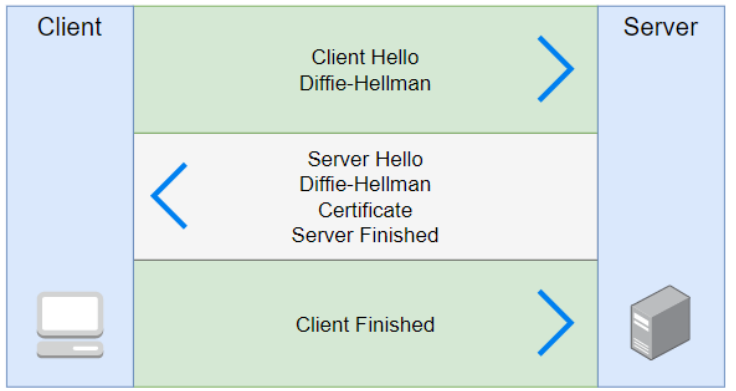
\includegraphics[width=\linewidth]{TLS_handshake.png}

\subsection{TLS Handshake - Steps}

\begin{concept}{TLS Handshake Overview}\\
    \begin{enumerate}
        \item Client and server negotiate crypto algorithms
        \item Client and server perform Diffie-Hellman
        \item Client and server generate handshake keys
        \item Server authenticates to client
        \item Client and server prove to one another that no one has altered previous messages
        \item Client and server generate data keys
    \end{enumerate}
\end{concept}

\subsection{TLS Session Resumption}

\begin{concept}{Session Resumption}\\
    If there is an existing TLS session between a client and a server application, additional TLS sessions can be established without any public key computations.
\end{concept}

\subsection{TLS Data Exchange}

\begin{KR}{TLS Data Processing}\\
    \paragraph{Step 1} Fragmentation
    \paragraph{Step 2} Encryption + prepend IV
    \paragraph{Step 3} Prepend Header
    
    A sequence number is used to ensure the order of all TLS records, when they arrive.
\end{KR}


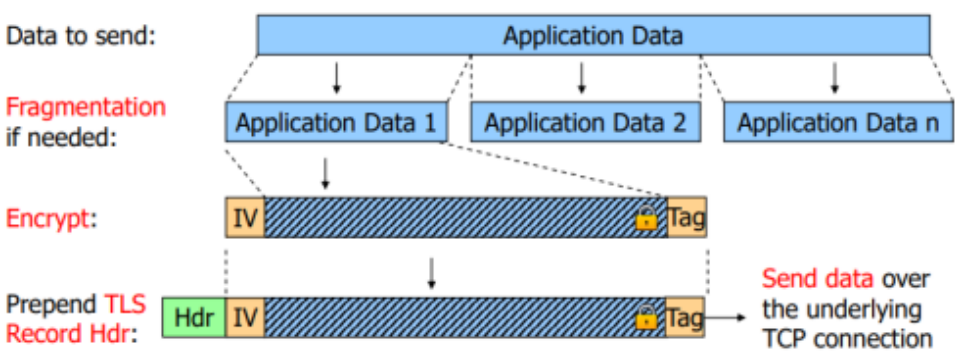
\includegraphics[width=\linewidth]{TLS_data_exchange.png}

\subsection{Cipher suites}

\begin{definition}{Cipher Suites}\\
    A set of cryptographic algorithms: "TLS\_AES\_128\_GCM\_SHA256"
\end{definition}

\subsection{State of TLS (Transport Layer Security - Wikipedia)}

\begin{remark}
    \begin{itemize}
        \item SSL 2.0, 3.0: major vulnerabilities supported by some servers
        \item TLS 1.0, 1.1: meh supported by 45\% of servers
        \item TLS 1.2: good supported almost universally
        \item TLS 1.3: good and fast
    \end{itemize}
    
    Latest browser versions are secure
    \begin{itemize}
        \item Only support TLS 1.0 – 1.3 and implement browser-side fixes for TLS 1.0 or simply disable it
        \item Most browsers don't support SSL 2.0 / 3.0 anymore
        \item TLS 1.3 is supported
    \end{itemize}
\end{remark}

\subsection{DTLS}

\begin{concept}{DTLS}\\
    Works on UDP instead of TCP
\end{concept}

\subsection{IPsec}

\begin{definition}{IPsec}\\
    \begin{itemize}
        \item Protects IP packets payload
        \item Protocol for network layer (IP)
        \item Security between two hosts
        \item Internet Key Exchange (IKE) in IPsec is like TLS handshake
    \end{itemize}
\end{definition}

\subsection{IP Packet Protection with ESP}

\begin{concept}{ESP}\\
    \begin{itemize}
        \item ESP = Encapsulating Security Payload
        \item ESP Provides confidentiality, authentication, and integrity
    \end{itemize}
\end{concept}

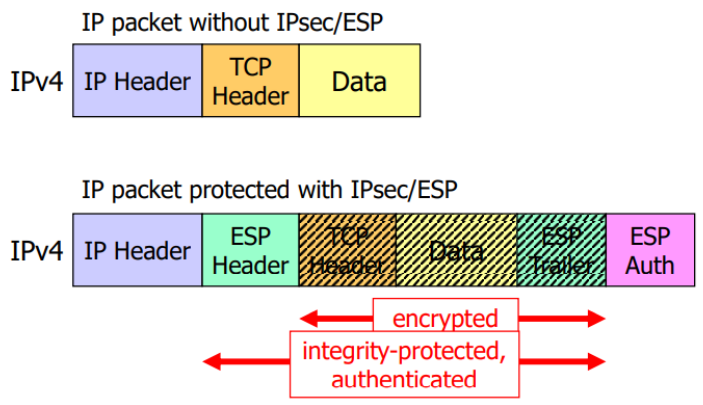
\includegraphics[width=\linewidth]{IPsec.png}

\subsection{IPSec Sequence Number}

\begin{concept}{Sequence Numbers}\\
    Order packets and drop duplicates

    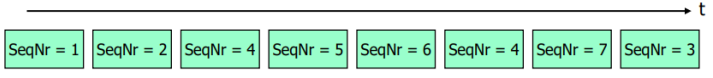
\includegraphics[width=\linewidth]{IPsec_sequence_nr.png}
\end{concept}